%% ============================================================
%% main.tex  — "The Necessity of Exploitation in Bayesian Optimization"
%% Compile:  pdflatex main → bibtex main → pdflatex main → pdflatex main
%% Overleaf: upload main.tex, all sec*.tex, references.bib, and the
%%           figures/ folder (exp_03_cd_diagram.png,
%%           exp_02_borehole_strategies.png, exp_02_ackley_strategies.png).
%% ============================================================
\documentclass[10pt, twocolumn]{article}

%% ------ Layout -----------------------------------------------
\usepackage[top=0.75in, bottom=0.85in, left=0.65in, right=0.65in,
            columnsep=0.2in]{geometry}
\usepackage{microtype}          % better line-breaking / spacing

%% ------ Math -------------------------------------------------
\usepackage{amsmath, amssymb}
\DeclareMathOperator*{\argmax}{arg\,max}  % used in §2

%% ------ Tables -----------------------------------------------
\usepackage{booktabs}           % \toprule / \midrule / \bottomrule
\usepackage{multirow}

%% ------ Graphics ---------------------------------------------
\usepackage{graphicx}
% Works for both local compilation (report/) and Overleaf upload.
\graphicspath{{./}{figures/}}

%% ------ Lists ------------------------------------------------
\usepackage{enumitem}           % [nosep] used in §1 and §4

%% ------ Bibliography (author–year, natbib) -------------------
\usepackage[round, authoryear]{natbib}
%% \citep{} → (Author, year)
%% \citet{} → Author (year)
%% \citeyear{} → year            [used in §5]

%% ------ Hyperlinks -------------------------------------------
\usepackage[colorlinks=true, linkcolor=blue, citecolor=blue, urlcolor=blue]{hyperref}

%% ------ Encoding (handles Unicode em-dash, ě, etc.) ----------
\usepackage[T1]{fontenc}
\usepackage[utf8]{inputenc}

%% ============================================================
%% Title block
%% ============================================================
\title{\textbf{The Necessity of Exploitation in Bayesian Optimization:\\
A Systematic Benchmark of Four Acquisition Strategies\\
on Six Problems}}

\author{Jianxiu Hou\\
  \texttt{jianxiuhou9@gmail.com}}

\date{June 2026}

%% ============================================================
\begin{document}

\maketitle
\thispagestyle{empty}

%% Abstract
% ============================================================
% Abstract
% ============================================================
\begin{abstract}
Bayesian optimization (BO) is widely used for expensive black-box
functions, where a Gaussian process (GP) surrogate drives an acquisition
function that balances exploration of uncertain regions against
exploitation of promising ones.
A fundamental open question is whether the GP's uncertainty estimate
alone—without any exploitation signal—is sufficient to outperform blind
random search.

I address this question with a systematic benchmark of four acquisition
strategies: Expected Improvement (EI), Upper Confidence Bound (UCB),
Uncertainty (maximum posterior standard deviation), and Random.
All four strategies share the same normalized GP surrogate and are
evaluated on six problems spanning dimensions 2 to 10, mixing classical
synthetic functions with physics-based engineering test functions.
Each strategy–problem pair is repeated over 10 independent seeds,
yielding 240 BO runs total.
A Friedman–Nemenyi non-parametric test ($N = 60$ blocks, $k = 4$)
provides statistically robust comparisons.

The Friedman test strongly rejects equal performance
($\chi^2(3) = 128.82$, $p = 9.73 \times 10^{-28}$).
Nemenyi post-hoc comparisons reveal two statistically separated
equivalence classes: balanced strategies $\{\text{EI, UCB}\}$
significantly outperform pure-exploration strategies
$\{\text{Uncertainty, Random}\}$ (all cross-class $p < 10^{-6}$),
while Uncertainty and Random are indistinguishable from each other
($p = 0.974$).
This Uncertainty–Random tie demonstrates that exploitation of the GP's
posterior mean—not the uncertainty estimate alone—is the necessary
condition for sample-efficient BO.
A secondary finding is that GP input normalization to known problem
bounds is a first-class engineering requirement on multi-scale problems:
omitting it degrades BO to random-search performance on Piston (7D),
while leaving the Random baseline unaffected, isolating the fault to
the surrogate.
\end{abstract}


%% §1 Introduction + §2 Background
% ============================================================
% §1  Introduction
% ============================================================
\section{Introduction}
\label{sec:introduction}

Bayesian optimization (BO) is the standard approach to optimizing
expensive black-box functions: objectives that are costly to evaluate,
return no gradients, and may be non-convex or multimodal
\citep{frazier2018tutorial,shahriari2016taking}.
Applications range from hyperparameter tuning in machine learning to
aerodynamic shape optimization, where each function evaluation can take
minutes to hours of computation or physical experiment.
BO sequentially builds a probabilistic surrogate model—typically a
Gaussian process (GP)—and uses an \emph{acquisition function} to decide
where to evaluate next.
The acquisition function must balance \emph{exploitation} (querying
where the surrogate predicts high values) against \emph{exploration}
(querying where the surrogate is uncertain, to reduce the risk of
missing a better region).

A natural question is whether the GP's uncertainty estimate alone is
sufficient to drive sample efficiency.
Purely uncertainty-driven sampling—selecting the point of maximum
posterior standard deviation—uses the GP's calibration to target
information gain, without any regard for whether the point is predicted
to have a high objective value.
If uncertainty-driven sampling outperforms blind random search, it would
suggest that the GP's uncertainty model, rather than the exploitation
signal, is the primary engine of BO's advantage.
If, on the other hand, it performs no better than random, it would
implicate exploitation as the necessary component.
Classical acquisition functions such as Expected Improvement (EI) and
Upper Confidence Bound (UCB) combine both signals; understanding which
component matters more is fundamental to designing and interpreting BO
algorithms.

I address this question through a systematic benchmark.
I evaluate four strategies—EI, UCB, Uncertainty (maximum posterior
standard deviation), and Random—on six benchmark problems spanning
dimensions 2 to 10 and two problem families: classical synthetic
functions and physics-based engineering test functions.
All strategies share the same GP surrogate and BO loop, so any
performance difference is attributable solely to the acquisition
function.
I use a Friedman–Nemenyi non-parametric statistical framework
\citep{demsar2006statistical} to draw conclusions robust to
non-Gaussian regret distributions.

\paragraph{Contributions.}
\begin{enumerate}[nosep]
  \item \textbf{Systematic 4-strategy benchmark.}
    I run 4 strategies $\times$ 6 problems $\times$ 10 seeds $= 240$
    BO runs under identical conditions and analyze results with a
    non-parametric test (Friedman + Nemenyi) rather than mean-only
    comparisons.
    The analysis reveals two statistically separated equivalence classes:
    balanced strategies \{EI, UCB\} and pure-exploration strategies
    \{Uncertainty, Random\}.

  \item \textbf{GP normalization is necessary on multi-scale engineering
    problems.}
    An experimental comparison on Piston (7D, inputs spanning
    approximately seven orders of magnitude) shows that omitting GP input
    normalization degrades BO to random-search performance, while the
    Random baseline is unaffected.
    This isolates the fault to the surrogate and validates the choice
    of explicit, bounds-based normalization.

  \item \textbf{Exploitation, not uncertainty, is the critical ingredient.}
    The statistical equivalence of Uncertainty and Random (Nemenyi
    $p = 0.974$) provides a controlled decomposition: the GP's
    posterior variance, used without the posterior mean, provides no
    measurable advantage over blind Sobol sampling.
    Exploitation of the GP mean is the necessary condition for
    sample-efficient BO.
\end{enumerate}

The remainder of the paper is organized as follows.
Section~\ref{sec:background} reviews the BO framework, the GP surrogate,
and related acquisition function families.
Section~\ref{sec:methods} details the experimental design, surrogate
implementation, and statistical methodology.
Section~\ref{sec:results} presents all benchmark results.
Section~\ref{sec:discussion} interprets the findings and discusses
limitations.
Section~\ref{sec:conclusion} concludes.

% ============================================================
% §2  Background
% ============================================================
\section{Background}
\label{sec:background}

\subsection{The Bayesian Optimization Loop}
\label{sec:bo-background}

Bayesian optimization solves $\max_{x \in \mathcal{X}} f(x)$ when $f$
is a black-box function that is expensive to evaluate, returns no
gradients, and may be multimodal \citep{frazier2018tutorial}.
The algorithm proceeds in two alternating steps.
First, a \emph{surrogate model} is fitted to all observations
$\{(x_i, y_i)\}_{i=1}^n$; it provides a posterior distribution over
$f$ with a calibrated mean $\mu(x)$ and variance $\sigma^2(x)$.
Second, an \emph{acquisition function} $\alpha(x)$ converts the
posterior into a scalar score at each candidate point; the next
evaluation location is $x_{n+1} = \argmax_{x \in \mathcal{X}} \alpha(x)$.
Solving the inner maximization is cheap because $\alpha$ is an
analytical function of the posterior.

BO is best suited to problems where: (i) each evaluation of $f$ is
expensive (minutes to hours), (ii) the dimensionality is low-to-moderate,
and (iii) gradients of $f$ are unavailable
\citep{frazier2018tutorial,shahriari2016taking}.

\subsection{Gaussian Process Surrogate}
\label{sec:gp-background}

A Gaussian process (GP) is a distribution over functions fully specified
by a mean function $m(x)$ and a positive-definite kernel
$k(x, x')$ \citep{frazier2018tutorial}.
After observing $n$ points, the GP posterior at a new location $x_*$
is Gaussian with
\[
  \mu(x_*) = k_*^\top (K + \sigma_n^2 I)^{-1} \mathbf{y},
  \qquad
  \sigma^2(x_*) = k(x_*, x_*) - k_*^\top (K + \sigma_n^2 I)^{-1} k_*,
\]
where $K_{ij} = k(x_i, x_j)$, $k_* = [k(x_i, x_*)]_i$, and
$\sigma_n^2$ is the noise variance.
The key computational cost is the $n\times n$ matrix inversion (or
Cholesky decomposition), which is $\mathcal{O}(n^3)$ and limits exact
GP inference to $n \lesssim 10^3$ observations \citep{shahriari2016taking}.

The kernel encodes smoothness assumptions about $f$.
I use the radial basis function (RBF) kernel with
\emph{automatic relevance determination} (ARD): one independent
lengthscale $\ell_j$ per input dimension $j$.
ARD allows the GP to learn which dimensions carry most of the variation
in $f$, effectively performing soft variable selection.
Kernel hyperparameters are fitted by maximizing the exact marginal
log-likelihood at each BO iteration.

\subsection{Acquisition Functions}
\label{sec:acq-background}

Acquisition functions trade off exploitation of high-mean regions
against exploration of high-variance regions.
All classical acquisition functions use both $\mu(x)$ and $\sigma(x)$;
the key difference is how they weight the two signals.

\paragraph{Expected Improvement (EI).}
$\alpha_{\mathrm{EI}}(x) = \mathbb{E}[\max(f(x) - f^+, 0)]$ where
$f^+ = \max_i y_i$ is the current best observation.
Under a GP this has the closed form
$\alpha_{\mathrm{EI}}(x) = \sigma(x)[\gamma\Phi(\gamma) + \phi(\gamma)]$
with $\gamma = (\mu(x) - f^+)/\sigma(x)$ \citep{frazier2018tutorial}.
EI is positive even when $\mu(x) < f^+$, provided $\sigma(x)$ is
large—this is why EI naturally explores uncertain regions.
EI has no finite-time regret guarantee.

\paragraph{Upper Confidence Bound (UCB).}
$\alpha_{\mathrm{UCB}}(x) = \mu(x) + \sqrt{\beta}\,\sigma(x)$.
The parameter $\beta$ directly controls the exploration–exploitation
trade-off.
Under a theory-motivated schedule $\beta_t \propto \log t$, GP-UCB
achieves sub-linear cumulative regret \citep{frazier2018tutorial}.
In practice a fixed $\beta$ is common; I use $\beta = 2$.

\paragraph{Pure-exploration strategies.}
Maximizing $\sigma(x)$ alone—without any $\mu(x)$ term—corresponds to
selecting the point about which the GP is most uncertain.
This pure-exploration strategy is useful as a controlled ablation: it
uses the GP's calibration machinery but discards all exploitation signal.
Blind random search serves as the weakest baseline.
De~Ath et al.~\citeyear{deAth2019greed} give a theoretical framing:
they show EI and UCB both lie on the exploration–exploitation Pareto
front in the ($\mu$, $\sigma$) plane, whereas maximum-$\sigma$ sampling
is off this front—it is Pareto-dominated in the exploitation dimension.
Their empirical results suggest this off-front position is
consequential in higher dimensions.

\subsection{Related Work}
\label{sec:related}

\paragraph{Comparative benchmarks.}
Several large-scale BO benchmarks have compared acquisition strategies.
Shahriari et al.~\citeyear{shahriari2016taking} review EI, UCB,
Thompson Sampling, and Entropy Search across diverse tasks, and conclude
that the choice of surrogate model typically matters more than the
fine-grained choice of acquisition function—a claim my normalization
experiment instantiates concretely.
De~Ath et al.~\citeyear{deAth2019greed} compare standard acquisition
functions against $\varepsilon$-greedy methods on ten synthetic benchmarks plus
real-world tasks, finding that simple greedy strategies are competitive
with EI and UCB in high dimensions.

\paragraph{Statistical methodology.}
\Citet{demsar2006statistical} argues that comparing classifiers—or, by
extension, optimization algorithms—over multiple datasets requires
non-parametric rank-based tests rather than mean-performance
comparisons, because regret distributions are typically non-Gaussian and
the null hypothesis of equal distributions is not testable with a single
paired $t$-test across datasets.
I adopt the Friedman–Nemenyi framework he recommends for exactly this
reason.


%% §3 Methods
% ============================================================
% §3  Methods
% ============================================================
\section{Methods}
\label{sec:methods}

\subsection{Bayesian Optimization Protocol}
\label{sec:protocol}

I follow the standard sequential BO protocol.
An initial design of $n_{\mathrm{init}} = 2d$ points is drawn via Sobol
quasi-random sampling, where $d$ is the problem dimensionality; Sobol
provides more uniform space-filling coverage than independent uniform
random draws.
After the initial design I run $T = 20$ sequential optimization
iterations.
At each step the GP surrogate is refitted to all accumulated observations,
the acquisition function is maximized to select one candidate point, and
the true objective is evaluated at that point.
All tensor computations use \texttt{torch.float64} to preserve GP
numerical stability.

\paragraph{Performance metric.}
Performance is measured by \emph{simple regret}
\[
  r_t = f^* - \max_{i \le t}\, y_i,
\]
where $f^*$ is the known optimal value and $y_i$ are observed function
values.
Because all six problems are framed as \emph{maximization},
$r_t \ge 0$ throughout every run and decreases toward zero as
the optimizer improves.

\paragraph{Experimental protocol.}
Each strategy–problem pair is evaluated across 10 independent random
seeds.
Acquisition functions are maximized using BoTorch's
\texttt{optimize\_acqf} with multi-start optimization
(\texttt{num\_restarts}\,$= 10$, \texttt{raw\_samples}\,$= 64$).

% ----------------------------------------------------------
\subsection{Gaussian Process Surrogate}
\label{sec:gp}

I use BoTorch's \texttt{SingleTaskGP}~\citep{balandat2020botorch} as
the surrogate: a Gaussian process with a radial basis function (RBF)
kernel equipped with automatic relevance determination (ARD), one
independent lengthscale per input dimension.
Kernel hyperparameters—lengthscales, output scale, and noise
variance—are fitted by maximizing the exact marginal log-likelihood
(MLL) at every iteration.

\paragraph{Input normalization.}
A critical design choice is to normalize GP inputs to the unit
hypercube $[0,1]^d$ and standardize outputs to zero mean and unit
variance before fitting.
I apply BoTorch's \texttt{Normalize(d,\,bounds=problem.bounds)} and
\texttt{Standardize(m=1)} transforms, using the \emph{known, fixed}
problem bounds rather than data-adaptive bounds.
Fixing the normalization range to the full search space prevents it
from drifting as observations accumulate, giving the GP a stable
length-scale calibration throughout the run.

The necessity of this choice was revealed empirically by the two
engineering problems.
Borehole and Piston have inputs spanning approximately seven orders of
magnitude (e.g.\ Piston's initial gas volume
$V_0 \in [0.002,\,0.010]\,\mathrm{m}^3$ alongside ambient pressure
$P_0 \in [90\,000,\,110\,000]\,\mathrm{Pa}$, a factor of roughly
$10^7$).
Without normalization, the GP cannot learn sensible per-dimension
lengthscales across these scales, causing EI and UCB to degrade to
random-search performance.
Table~\ref{tab:normalization} shows the effect on Piston, where the
controlled comparison is cleanest: adding normalization reduces EI's
mean final regret from $0.41$ to $0.019$ (${\approx}20{\times}$) and
UCB's from $0.39$ to $0.0019$ (${\approx}200{\times}$), while the
Random baseline—which makes no GP calls—remains unchanged at
${\approx}0.40$.
The unchanged Random performance isolates the fault squarely to the
surrogate, not the problem formulation.

\begin{table}[h]
\centering
\caption{Effect of GP input normalization on mean final regret on
  Piston (7D), 10 seeds.  Random is unchanged because it does not use
  the GP, confirming the fault is in the surrogate.}
\label{tab:normalization}
\begin{tabular}{lccc}
\toprule
Strategy & Before norm. & After norm. & Improvement \\
\midrule
EI       & 0.41  & \textbf{0.019}  & ${\approx}20{\times}$  \\
UCB      & 0.39  & \textbf{0.0019} & ${\approx}200{\times}$ \\
Random   & 0.40  & 0.41            & —                      \\
\bottomrule
\end{tabular}
\end{table}

% ----------------------------------------------------------
\subsection{Acquisition Strategies}
\label{sec:strategies}

I benchmark four strategies that together span the full
exploration–exploitation spectrum (Table~\ref{tab:strategies}).

\paragraph{Expected Improvement (EI).}
\[
  \alpha_{\mathrm{EI}}(x)
    = \mathbb{E}\!\left[\max\!\bigl(f(x) - f^+,\, 0\bigr)\right],
\]
where $f^+ = \max_i y_i$ is the current best observed value.
Under a GP surrogate this has the closed form
$\alpha_{\mathrm{EI}}(x) =
  \sigma(x)\!\left[\gamma(x)\Phi(\gamma(x)) + \phi(\gamma(x))\right]$,
with $\gamma(x) = (\mu(x) - f^+)/\sigma(x)$, where $\Phi$ and $\phi$
are the standard Gaussian CDF and PDF.
EI rewards both a high posterior mean (exploitation) and a high
posterior variance (exploration); neither component alone is
sufficient to generate positive EI.
Implemented via \texttt{botorch.acquisition.ExpectedImprovement} with
\texttt{best\_f = train\_y.max()}.

\paragraph{Upper Confidence Bound (UCB).}
\[
  \alpha_{\mathrm{UCB}}(x) = \mu(x) + \sqrt{\beta}\,\sigma(x),
  \quad \beta = 2.
\]
The $\beta$ parameter controls the exploration–exploitation
trade-off.
Unlike EI, GP-UCB has finite-time regret guarantees under appropriate
$\beta$ schedules~\citep{frazier2018tutorial}.
Implemented via \texttt{botorch.acquisition.UpperConfidenceBound}.

\paragraph{Uncertainty (pure exploration).}
\[
  \alpha_{\mathrm{Unc}}(x) = \sigma(x).
\]
This strategy selects the point of maximum posterior standard
deviation, entirely ignoring the posterior mean.
It is the pure-exploration extreme of the spectrum: it uses the same
GP as EI and UCB but discards all exploitation signal.
Its inclusion allows me to isolate whether the GP's uncertainty
estimate \emph{alone}—without any mean information—is sufficient to
outperform blind search.
Implemented via \texttt{botorch.acquisition.PosteriorStandardDeviation}.

\paragraph{Random (baseline).}
Points are drawn from a Sobol sequence within the search bounds at
every iteration; the GP is never called.
This is the weakest baseline that any data-efficient strategy must
surpass.

\begin{table}[h]
\centering
\caption{The four acquisition strategies and their position on the
  exploration–exploitation spectrum.}
\label{tab:strategies}
\begin{tabular}{llcc}
\toprule
Strategy & Acquisition & Uses $\mu$? & Uses $\sigma$? \\
\midrule
EI          & ExpectedImprovement  & \checkmark             & \checkmark \\
UCB         & UpperConfidenceBound & \checkmark             & \checkmark \\
Uncertainty & PosteriorStdDev      & \phantom{\checkmark}   & \checkmark \\
Random      & Sobol sampling       & \phantom{\checkmark}   & \phantom{\checkmark} \\
\bottomrule
\end{tabular}
\end{table}

% ----------------------------------------------------------
\subsection{Problem Suite}
\label{sec:problems}

I benchmark on six functions spanning dimensions $d \in \{2,6,7,8,10\}$
across two categories (Table~\ref{tab:problems}).

\begin{table*}[t]
\centering
\caption{Benchmark problem suite.  All problems are framed as
  maximization; simple regret is $f^* - \text{best observed}$.
  Engineering optimal values are derived from exhaustive corner search
  ($2^d$ vertices) rather than random sampling, which systematically
  undershoots vertex maxima on monotone functions (see
  Section~\ref{sec:gp}).}
\label{tab:problems}
\begin{tabular}{llcll}
\toprule
Problem & Type & $d$ & Domain & $f^*$ \\
\midrule
Branin          & Synthetic    & 2  & standard          & $-0.3979$ \\
Six-Hump Camel  & Synthetic    & 2  & $[-3,3]\times[-2,2]$ & $1.0316$ \\
Hartmann-6      & Synthetic    & 6  & $[0,1]^6$         & $3.3224$  \\
Piston          & Engineering  & 7  & multi-scale       & $1.20$    \\
Borehole        & Engineering  & 8  & multi-scale       & $310.0$   \\
Ackley-10D      & Synthetic    & 10 & $[-5,5]^{10}$     & $0.0$     \\
\bottomrule
\end{tabular}
\end{table*}

\textbf{Synthetic problems} (Branin, Six-Hump Camel, Hartmann-6,
Ackley-10D) wrap BoTorch's built-in test functions with
\texttt{negate=True} to convert minimization to maximization;
optimal values are analytically known.
The Ackley bounds are narrowed from BoTorch's default
$[-32.768, 32.768]^{10}$ to the literature-standard $[-5, 5]^{10}$.

\textbf{Engineering problems} model physical systems with inputs at
physically meaningful, heterogeneous scales.
\emph{Borehole} (8D) models water flow through a borehole; inputs
include borehole radius, hydraulic transmissivities, water-table
elevations, and aquifer conductivity, sourced from SMT's
\texttt{WaterFlow}.
\emph{Piston} (7D) models piston cycle time as a function of mass $M$,
surface area $S$, initial gas volume $V_0$, spring stiffness $k$,
atmospheric pressure $P_0$, ambient temperature $T_a$, and gas
temperature $T_0$ \citep{surjanovic2013virtual}.
Piston is absent from the SMT version used, so it is implemented
manually from the standard closed-form formula.
For both engineering functions the global maximum lies at a box vertex;
optimal values are obtained by exhaustive corner evaluation
($2^8 = 256$ and $2^7 = 128$ vertices respectively) and a small
conservative buffer to guarantee non-negative simple regret.

% ----------------------------------------------------------
\subsection{Statistical Methodology}
\label{sec:stats}

With four strategies and six problems, I require a comparison
framework that is robust to non-Gaussian, heavy-tailed regret
distributions and avoids the inflated type-I error of repeated
pairwise $t$-tests.
Following \citet{demsar2006statistical}, I use the Friedman rank test
with Nemenyi post-hoc pairwise comparisons.

\paragraph{Friedman test.}
Each (problem, seed) pair forms one block; the four strategies are
ranked by final regret within each block, rank 1 indicating best.
This yields $N = 60$ blocks (6 problems $\times$ 10 seeds) and
$k = 4$ strategies.
The Friedman statistic tests the null hypothesis that all strategies
have equal expected rank.

\paragraph{Nemenyi post-hoc test.}
On rejection of the Friedman null, all $\binom{4}{2} = 6$ pairwise
comparisons are performed using Nemenyi's test at $\alpha = 0.05$
\citep{terpilowski2019scikit}.
Two strategies are deemed \emph{statistically indistinguishable} when
their average-rank difference is less than the critical difference
\[
  \mathrm{CD}
    = q_\alpha \sqrt{\frac{k(k+1)}{6N}}
    = q_{0.05}\sqrt{\frac{4 \times 5}{6 \times 60}},
\]
where $q_\alpha$ is the critical value from the Studentized range
distribution (divided by $\sqrt{2}$); $\mathrm{CD} \approx 0.61$ for
$k=4$, $N=60$, $\alpha=0.05$.
Results are visualized as a Critical Difference (CD) diagram
(Figure~\ref{fig:cd}), where horizontal bars connect strategies that
are not significantly different from one another.
The CD value is computed analytically inside the plotting function to
remain correct under any change to $N$ or $k$.


%% §4 Results
% ============================================================
% §4  Results
% ============================================================
\section{Results}
\label{sec:results}

I report three complementary views of the benchmark: the omnibus
statistical ranking, per-problem median regret, and regret trajectories.
Together they tell a consistent story: the 240 BO runs partition the
four strategies into two statistically separated equivalence classes.

% ----------------------------------------------------------
\subsection{Omnibus Statistical Test}
\label{sec:friedman}

The Friedman test strongly rejects the null hypothesis of equal expected
ranks across the four strategies:
$\chi^2(3) = 128.82$, $p = 9.73 \times 10^{-28}$ ($N = 60$ blocks,
$k = 4$).
Average ranks are
UCB $= 1.39$, EI $= 1.76$, Uncertainty $= 3.38$, Random $= 3.48$.

The rank ordering partitions into two well-separated groups.
The gap between EI (1.76) and Uncertainty (3.38) is $1.62$, more than
two and a half times the critical difference $\mathrm{CD} = 0.61$.
Within each group the gaps are small: UCB and EI differ by $0.37$
(below CD), and Uncertainty and Random differ by $0.10$ (far below CD).

% ----------------------------------------------------------
\subsection{Nemenyi Pairwise Comparisons}
\label{sec:nemenyi}

All six pairwise Nemenyi comparisons at $\alpha = 0.05$ are reported in
Table~\ref{tab:nemenyi} and visualized in the Critical Difference diagram
(Figure~\ref{fig:cd}).

\begin{table*}[t]
\centering
\caption{Nemenyi post-hoc $p$-values.
  NS = not significant at $\alpha = 0.05$; ${}^{***}$ = $p < 10^{-6}$.
  Two distinct equivalence classes emerge: \{UCB, EI\} and
  \{Uncertainty, Random\}.}
\label{tab:nemenyi}
\begin{tabular}{lcccc}
\toprule
         & UCB     & EI      & Uncertainty & Random \\
\midrule
UCB      & —       & 0.404 \scriptsize{(NS)} & $<\!10^{-6}$ ${}^{***}$ & $<\!10^{-6}$ ${}^{***}$ \\
EI       &         & —       & $<\!10^{-6}$ ${}^{***}$ & $<\!10^{-6}$ ${}^{***}$ \\
Uncertainty &      &         & —           & 0.974 \scriptsize{(NS)} \\
Random   &         &         &             & — \\
\bottomrule
\end{tabular}
\end{table*}

The results define two equivalence classes:
\begin{itemize}[nosep]
  \item \textbf{Balanced strategies}: \{UCB, EI\} — statistically
    indistinguishable from each other ($p = 0.404$), both significantly
    better than the pure-exploration strategies ($p < 10^{-6}$).
  \item \textbf{Pure-exploration strategies}: \{Uncertainty, Random\} —
    statistically indistinguishable from each other ($p = 0.974$), both
    significantly worse than the balanced strategies ($p < 10^{-6}$).
\end{itemize}

The most striking result is the Uncertainty–Random tie.
Uncertainty selects points by maximizing posterior standard deviation
using the same fitted GP as EI and UCB; it is not a blind strategy.
Yet its rank ($3.38$) is statistically indistinguishable from Random
($3.48$, $p = 0.974$).
This isolates the contribution of exploitation: the GP's uncertainty
estimate, used \emph{without} the posterior mean, provides no
measurable advantage over blind Sobol sampling.

\begin{figure*}[t]
  \centering
  
\includegraphics[width=0.82\linewidth]{figures/exp_03_cd_diagram.png}
  \caption{Critical Difference diagram ($\alpha = 0.05$, $k = 4$,
    $N = 60$, $\mathrm{CD} = 0.61$).
    Horizontal bars connect strategies that are not significantly
    different.  Two separate cliques are visible: \{UCB, EI\}
    (left, lower ranks = better) and \{Uncertainty, Random\}
    (right, higher ranks = worse).}
  \label{fig:cd}
\end{figure*}

% ----------------------------------------------------------
\subsection{Per-Problem Median Regret}
\label{sec:per-problem}

Table~\ref{tab:median} reports median final regret across 10 seeds for
each problem–strategy pair.
I report median rather than mean because several seeds produce
outlier-high regret on certain problem–strategy combinations; for
example, EI on Borehole has a mean final regret of $8.63$ (inflated by
two outlier seeds) but a median of only $2.41$.
Median is more representative of typical performance and robust to
heavy-tailed distributions.

\begin{table*}[t]
\centering
\caption{Median final simple regret after 20 iterations, 10 seeds.
  Bold = best per row.  Ordered by dimension.
  All problems are maximization; lower regret is better.}
\label{tab:median}
\begin{tabular}{lcccc}
\toprule
Problem ($d$) & EI & UCB & Uncertainty & Random \\
\midrule
Branin (2)       & 0.026 & \textbf{0.015} & 2.676 & 0.920 \\
SixHumpCamel (2) & \textbf{0.057} & 0.287 & 0.936 & 0.924 \\
Hartmann-6 (6)   & \textbf{0.183} & 0.254 & 1.913 & 1.802 \\
Piston (7)       & 0.016 & \textbf{0.001} & 0.033 & 0.395 \\
Borehole (8)     & 2.409 & \textbf{0.424} & 5.747 & 111.642 \\
Ackley-10D (10)  & \textbf{3.800} & 4.295 & 8.441 & 8.272 \\
\midrule
Avg.\ rank & 1.76 & \textbf{1.39} & 3.38 & 3.48 \\
\bottomrule
\end{tabular}
\end{table*}

Several patterns are visible across the table.
First, the balanced strategies (EI, UCB) lead on every single problem;
the pure-exploration strategies (Uncertainty, Random) never win a row.
Second, the magnitude of the advantage varies substantially with problem
structure.
On Borehole (8D, engineering), UCB's median regret ($0.42$) is
$263\times$ lower than Random's ($111.6$), reflecting the structured,
near-monotone response surface that a well-calibrated GP can exploit.
On Ackley-10D (synthetic, highly multimodal), EI's median ($3.80$)
is only $2.2\times$ lower than Random's ($8.27$), consistent with
the curse of dimensionality degrading GP calibration at this budget.
Third, among the balanced strategies, neither EI nor UCB consistently
dominates: UCB ranks first on four of six problems, EI on two, and
their average ranks (1.39 vs.\ 1.76) are not significantly different
(Nemenyi $p = 0.404$).

% ----------------------------------------------------------
\subsection{Regret Trajectories}
\label{sec:trajectories}

Figures~\ref{fig:borehole} and~\ref{fig:ackley} show mean regret
trajectories ($\pm$ one standard deviation) across seeds for the two
most contrasting problems.

\begin{figure}[tb]
  \centering
  
\includegraphics[width=\linewidth]{figures/exp_02_borehole_strategies.png}
  \caption{Mean regret $\pm$ std over 20 iterations on Borehole (8D).
    EI and UCB converge rapidly while Uncertainty and Random show
    negligible improvement.
    The large EI std band is driven by two outlier seeds with elevated
    final regret, inflating the mean well above the median ($8.63$
    vs.\ $2.41$).}
  \label{fig:borehole}
\end{figure}

\begin{figure}[tb]
  \centering
  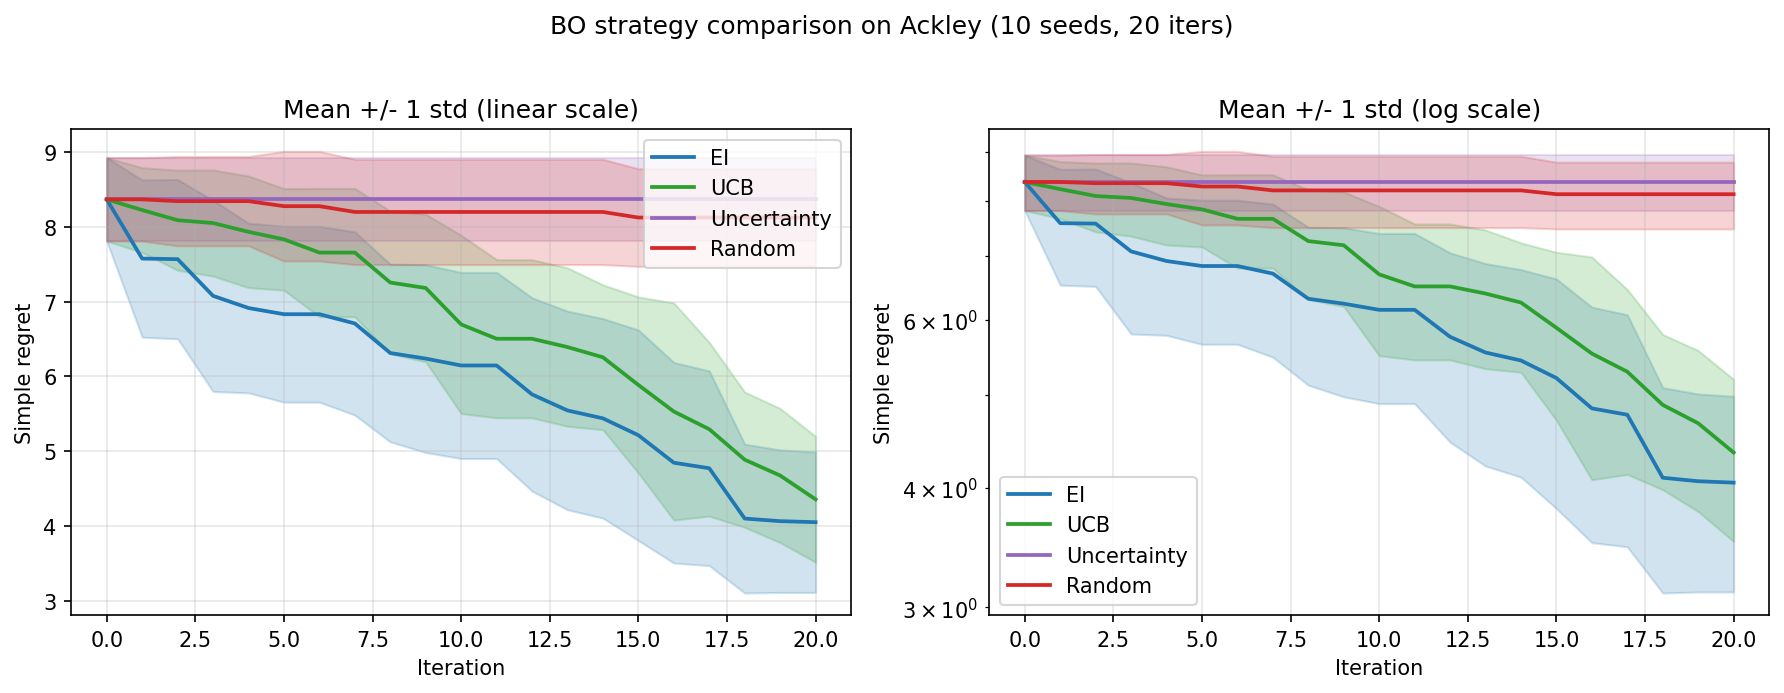
\includegraphics[width=\linewidth]{figures/exp_02_ackley_strategies.png}
  \caption{Mean regret $\pm$ std over 20 iterations on Ackley-10D.
    All four strategies remain at high regret; EI and UCB show a
    marginal but consistent advantage over pure-exploration strategies.
    The narrow gap between balanced and pure-exploration strategies
    illustrates dimensionality-driven degradation of GP calibration.}
  \label{fig:ackley}
\end{figure}

% ----------------------------------------------------------
\subsection{Effect of Dimensionality}
\label{sec:dimension}

To quantify how the EI–Random gap changes with dimensionality I use
mean final regret, which captures tail behavior that median suppresses.
On Branin (2D), EI achieves a mean regret of $0.034$ against Random's
$1.58$, a ${\approx}47{\times}$ advantage.
On Ackley-10D, EI achieves $4.05$ against Random's $8.13$, a
${\approx}2{\times}$ advantage—a more than 20-fold reduction in relative
gain over eight additional dimensions.

This collapse in advantage is consistent with the theoretical analysis
in \citet{shahriari2016taking}: in high dimensions the GP surrogate
requires exponentially more observations to achieve accurate uncertainty
estimates, and the 20-iteration budget used here is far from sufficient
to cover the $[-5, 5]^{10}$ search space.
The Ackley function has no low-effective-dimensionality structure that
could be exploited through embeddings or variable selection, making it a
worst-case scenario for GP-based BO at this budget.


%% §5 Discussion + §6 Conclusion
% ============================================================
% §5  Discussion
% ============================================================
\section{Discussion}
\label{sec:discussion}

\subsection{Exploitation Is the Critical Ingredient}
\label{sec:exploitation}

The most consequential result is not that EI and UCB outperform Random—
that is expected—but that Uncertainty is statistically indistinguishable
from Random ($p = 0.974$, average ranks $3.38$ vs.\ $3.48$).
Uncertainty is not a blind strategy: it fits the same GP as EI and UCB
at every iteration and selects the point of maximum posterior standard
deviation.
Yet its rank matches that of blind Sobol sampling across 60
(problem, seed) blocks.

This isolates where the value of BO lies.
Uncertainty and Random share one characteristic: neither uses the GP's
posterior mean.
EI and UCB share the complementary characteristic: both combine the
posterior mean with the posterior variance.
The equivalence classes therefore provide a clean experimental
decomposition—the GP's uncertainty estimate alone is insufficient;
exploitation of the mean is the necessary component.

Two independent lines of theory predict this outcome.
De~Ath et al.~\citeyear{deAth2019greed} recast acquisition function
selection as a bi-objective problem: they show that EI and UCB both
select points on the exploration–exploitation Pareto front, whereas a
strategy that uses only $\sigma(x)$ (the pure-exploration extreme) sits
off this front in the exploitation dimension.
Shahriari et al.~\citeyear{shahriari2016taking} observe that acquisition
functions matter, but caution against over-indexing on any single one;
their framing implies that the \emph{balance} between the two GP signals
is what separates effective from ineffective acquisition strategies.
Both predictions are borne out by the Uncertainty–Random equivalence.

\subsection{EI and UCB Are Interchangeable at This Budget}
\label{sec:ei-ucb}

Within the balanced-strategy class, EI and UCB are statistically
indistinguishable (Nemenyi $p = 0.404$), despite different theoretical
properties: UCB has finite-time regret guarantees under appropriate
$\beta$ schedules, whereas EI has no such guarantee.
The per-problem medians echo this: UCB leads on four of six problems, EI
on two, with no consistent pattern by problem type or dimension.

De~Ath et al.~\citeyear{deAth2019greed} provide a mechanistic
explanation: both EI and UCB lie on the exploration–exploitation Pareto
front, so they explore at similar rates; any residual difference is
smaller than the problem-to-problem and seed-to-seed variance at a
20-iteration budget.
Shahriari et al.~\citeyear{shahriari2016taking} reinforce this with a
broader observation: the surrogate model's adequacy typically dominates
the fine-grained acquisition choice.
The EI–UCB equivalence is therefore not a sample-size failure but the
expected outcome of using two well-designed balanced strategies on the
same adequate surrogate.

\subsection{GP Normalization as a First-Class Methodological Result}
\label{sec:normalization}

The GP normalization result warrants discussion beyond a footnote in the
Methods section.
The initial experiment on Piston (7D) showed EI and UCB performing at
random-search level—plausible only if the surrogate were failing.
Piston's inputs span approximately seven orders of magnitude—initial gas
volume $V_0 \in [0.002,\,0.010]\,\mathrm{m}^3$ alongside ambient
pressure $P_0 \in [90\,000,\,110\,000]\,\mathrm{Pa}$—so an
un-normalized GP cannot learn meaningful per-dimension lengthscales.
Adding \texttt{Normalize} and \texttt{Standardize} recovered ${\approx}20\times$
improvement for EI and ${\approx}200\times$ for UCB, while Random—
which bypasses the GP—remained unchanged, isolating the fault to the
surrogate.

This finding directly instantiates Shahriari et al.'s
\citeyear{shahriari2016taking} claim that surrogate adequacy dominates
acquisition choice: the problem was not that EI or UCB was the wrong
acquisition function, but that the surrogate itself was miscalibrated.
It also underscores a practical lesson for engineers deploying BO on
real systems: physical inputs with heterogeneous scales require explicit
normalization to the known search bounds, not data-adaptive bounds that
drift as observations accumulate.

\subsection{Limitations}
\label{sec:limitations}

\paragraph{Budget.}
The 20-iteration budget is appropriate for expensive black-box
functions~\citep{frazier2018tutorial}, but it is tight relative to the
10D Ackley search space.
At this budget, no strategy explores more than a small fraction of
$[-5, 5]^{10}$, which suppresses the EI–Random advantage from $47\times$
on 2D Branin to $2\times$ on 10D Ackley and limits conclusions about
asymptotic performance.
Longer-horizon experiments would be needed to determine whether
balanced strategies accumulate a growing advantage in high dimensions
or plateau.

\paragraph{Fixed $\beta$ for UCB.}
I use a fixed $\beta = 2$ throughout, which does not follow the
theory-motivated schedule $\beta_t \propto \log t$ under which GP-UCB's
regret guarantees hold~\citep{frazier2018tutorial}.
A theory-consistent $\beta$ schedule may widen or narrow the EI–UCB gap;
I cannot rule out this effect from the current experiment.

\paragraph{Sequential-only evaluation.}
All results use sequential ($q = 1$) BO.
Batch acquisition ($q > 1$, e.g.\ qEI) is important in practice when
multiple evaluations can run in parallel, and the relative performance of
strategies may differ in the batch setting.

\paragraph{Synthetic and physics-emulator problems only.}
The benchmark includes six analytic or closed-form problems.
Real engineering simulations—such as CFD or aerodynamic design codes—may
exhibit noise, discontinuities, or constraint violations not present
here.
Whether the two-clique finding persists on black-box simulation outputs
remains an open question.

% ============================================================
% §6  Conclusion
% ============================================================
\section{Conclusion}
\label{sec:conclusion}

I benchmarked four acquisition strategies—EI, UCB, Uncertainty, and
Random—on six problems spanning dimensions 2 to 10 and two problem
families (synthetic and engineering), using a Friedman–Nemenyi
non-parametric framework with $N = 60$ blocks.
The results converge on two findings.

First, the 240 BO runs partition cleanly into two equivalence classes:
balanced strategies \{EI, UCB\} are statistically superior to
pure-exploration strategies \{Uncertainty, Random\}, with all
cross-class Nemenyi $p$-values below $10^{-6}$ and an inter-class rank
gap of $1.62 \gg \mathrm{CD} = 0.61$.
The Uncertainty–Random tie ($p = 0.974$) is the sharpest statement of
this result: using a GP for exploration only, without any exploitation
of the posterior mean, provides no measurable advantage over blind
random search.

Second, GP normalization to the known problem bounds is a
first-class engineering requirement on multi-scale problems.
Without it, BO on Piston degraded to random-search performance;
restoring it recovered one to two orders of magnitude in final regret.
This confirms the theoretical expectation that surrogate adequacy
dominates the acquisition-function choice and highlights a pitfall
specific to physical systems with heterogeneous input scales.


%% References
\bibliographystyle{plainnat}
\bibliography{references}

\end{document}
